\documentclass[sigconf,review]{acmart}
% \settopmatter{printfolios=true}
% \documentclass[review]{acmart}\settopmatter{printfolios=true}
\usepackage{amssymb}
\usepackage{amsthm}
\usepackage{graphicx}
\usepackage{amsmath}
\usepackage{mathptmx}
\usepackage{mathtools}
\usepackage{stmaryrd}
% \usepackage{adjustbox}
\usepackage{hyperref}
\usepackage{alltt}
\usepackage{url}
\usepackage{float}
% \usepackage{minipage-marginpar}
\usepackage{style/utils}
\usepackage{style/code}
\usepackage{style/proof}
\usepackage{style/keywords}
\usepackage{style/layout}
\usepackage{style/judgements}

% for combinator pictures
\usepackage{tikz}
\usepackage{pgfplots}
\usetikzlibrary{shapes,arrows}
\usepackage[outputdir={out/}]{dot2texi}

\setcopyright{none}
% \bibliographystyle{ACM-Reference-Format}
% \citestyle{acmauthoryear}

% -----------------------------------------------------------------------------
\begin{document}

\title{Machine Fusion (Appendices)}
\subtitle{Merging merges, more or less}

\author{Amos Robinson}
\affiliation{Ambiata and UNSW (Australia)}
\email{amosr@cse.unsw.edu.au}

\author{Ben Lippmeier}
\affiliation{Digital Asset and UNSW (Australia)}
\email{benl@ouroborus.net}

\makeatactive
\maketitle

\appendix

\vspace{5em}
This document contains technical appendices to the main paper.

\begin{itemize}
\item Appendix \ref{s:FiniteDetails} -- Finite Streams
\item Appendix \ref{s:ResultSize}    -- Result Size
\item Appendix \ref{s:Combinators}   -- Combinators
\end{itemize}

%!TEX root = ../Main.tex
\eject
\appendix

\section{Finite streams}
\label{s:FiniteDetails}

This appendix briefly describes the finite streams extension, showing the changes to instructions and the fusion algorithm.
The finite evaluation rules are not shown, as the changes follow the same structure as the changes to the fusion algorithm.

\begin{figure}
\begin{tabbing}
MMMMMM \TABDEF @MMMMM@  \TABSKIP $\Chan$ \TABSKIP $\Chan$ \TABSKIP $\Next$ \TABSKIP \kill
\Instr
    \> ::=\> @push@  \> \Chan  \> \Exp  \> \Next \\
    \TABALT  @drop@  \> \Chan  \>       \> \Next \\
    \TABALT  @case@  \> \Exp   \> \Next \> \Next \\
    \TABALT  @jump@  \>        \>       \> \Next \\
    \\
    \TABALT  @pull@  \> \Chan  \> \Var  \> \Next \> \Next \\
    \TABALT  @close@ \> \Chan  \>       \> \Next \\
    \TABALT  @exit@ 
\\
\\
$\InputState_F$ \> ::=  \> ~~~ $@none@_F ~|~ @pending@_F ~|~ @have@_F ~|~ @closed@_F$
\end{tabbing}
\caption{Finite instructions}
\label{fig:Finite:Instr}
\end{figure}

Figure~\ref{fig:Finite:Instr} shows the grammar for instructions and the static input state. The first group of instructions containing @push@, @drop@, @case@ and @jump@ are unchanged.

The @pull@ instruction is modified to have two output labels, similar to @case@. The first, the success branch, is used when the input stream is still open and pulling succeeds, in which case the variable is set to the pulled value as before. The second output label, the closed branch, is used when the input stream has been closed, and the variable is not written to. This new @pull@ is analogous to a @pull@ followed by a @case@ in the infinite stream version.

The @close@ instruction is used by a pushing process to close or end an output stream. Any subsequent pulls from this channel in other processes will take the closed branch. After an output channel is closed, it cannot be pushed to and remains closed forever.

Finally, the @exit@ instruction is used once a process is finished with all its streams, and has nothing left to do. All output streams must be closed before the process finishes. This instruction has no output labels, as there is nothing further to execute.

Also in Figure~\ref{fig:Finite:Instr}, the static input state used for fusion ($\InputState_F$) must now track closed streams. The new constructor $@closed@_F$ denotes that the stream is closed, while the rest is unchanged.

For the fusion algorithm, the top-level function $\ti{fusePair}$ remains unchanged. The functions $\ti{outlabels}$ and $\ti{swaplabels}$ are not shown as they are easily modified by adding cases for the new instructions.

Figure~\ref{fig:Finite:tryStepPair} shows the modified $\ti{tryStepPair}$ function. This function uses the same heuristics to decide which process to execute when both can progress, but now that the processes can finish with @exit@, we must take care to only finish the fused process once \emph{both} source processes are finished. The (DeferExit1) and (DeferExit2) clauses achieve this by forcing the other process to run if one is an @exit@. Once both processes are finished, both new clauses will fail while (DeferPull1) succeeds, using the @exit@ from the first process. Another way to think of this is that if either process has work to do, the fused process still has work to do.

\begin{figure}
\begin{tabbing}
M \= M \= M \= MMMMMMMMMMMMMMMMMMM \= \kill
$\ti{tryStepPair} ~:~ \ChanTypeMap$ \\
\> \> $\to \Label_1 \to \Instr$ ~~~
            $\to \Label_1 \to \Instr$ \\
\> \> $\to \Maybe~\Instr$ \\
$\ti{tryStepPair} ~\cs~l_p~i_p~l_q~i_q$ \\

\> $~|~i_p'~\in~\ti{tryStep}~\cs~l_p~i_p~l_q ~\wedge~ i_q'~\in~\ti{tryStep}~\cs~l_q~i_q~l_p$ \\
\> ~~ $\wedge~@exit@~\not\in~i_p'$ 
   ~~~~~ $\to~i_p'$ 
\> \> \> \note{DeferExit1} 
\\[0.5ex]

\> $~|~i_p'~\in~\ti{tryStep}~\cs~l_p~i_p~l_q ~\wedge~i_q'~\in~\ti{tryStep}~\cs~l_q~i_q~l_p$ \\
\> ~~ $\wedge~@exit@~\not\in~i_q'$ 
   ~~~~~ $\to~\ti{swaplabels}~i_q'$ 
\> \> \> \note{DeferExit2} 
\\[0.5ex]


\> $~|~i_p'~\in~\ti{tryStep}~\cs~l_p~i_p~l_q ~\wedge~@jump@~(l,u)~\in~i_p'$ \\
\> $\to~i_p'$
\> \> \> \note{PreferJump1} 
\\[0.5ex]

\> $~|~i_q'~\in~\ti{tryStep}~\cs~l_q~i_q~l_p ~\wedge~@jump@~(l,u)~\in~i_q'$ \\
\> $\to~\ti{swaplabels}~i_q'$ 
\> \> \> \note{PreferJump2}
\\[0.5ex]

\> $~|~i_p'~\in~\ti{tryStep}~\cs~l_p~i_p~l_q ~\wedge~ i_q'~\in~\ti{tryStep}~\cs~l_q~i_q~l_p$ \\
\> ~~ $\wedge~@pull@~c~x~(l,u)~\not\in~i_p'$ 
   ~~~~~ $\to~i_p'$ 
\> \> \> \note{DeferPull1} 
\\[0.5ex]

\> $~|~i_p'~\in~\ti{tryStep}~\cs~l_p~i_p~l_q ~\wedge~i_q'~\in~\ti{tryStep}~\cs~l_q~i_q~l_p$ \\
\> ~~ $\wedge~@pull@~c~x~(l,u)~\not\in~i_q'$ 
   ~~~~~ $\to~\ti{swaplabels}~i_q'$ 
\> \> \> \note{DeferPull2} 
\\[0.5ex]

\> $~|~i_p'~\in~\ti{tryStep}~\cs~l_p~i_p~l_q$ ~~~~~ $\to~i_p'$ 
\> \> \> \note{Run1} 
\\[0.5ex]

\> $~|~i_q'~\in~\ti{tryStep}~\cs~l_q~i_q~l_p$ ~~~~~ $\to~\ti{swaplabels}~i_q'$
\> \> \> \note{Run2} \\


\end{tabbing}
\caption{Fusion step coordination for a pair of processes.}
\label{fig:Finite:tryStepPair}
\end{figure}

Figure~\ref{fig:Finite:tryStep} shows the modified $\ti{tryStep}$ function.
The clauses for the unchanged instructions @push@, @drop@, @case@ and @jump@ remain unchanged; these are reordered to the top of the function.

The @pull@ clauses use $l'_o$ for the open output label, and $l'_c$ for the closed label.
Clause (LocalPull) now uses two output labels, and leaves the other process as-is.

Clause (SharedPull) applies when the channel state is @pending@, meaning there is already a value available. This means that the channel is not yet closed, and the success branch can be taken.

Clause (SharedPullInject) applies when both processes need to pull from a shared input. As before, we execute a real @pull@, this time with two branches. In the success branch, the input states are set to @pending@ as before. In the closed branch, the input states are set to @closed@ so the next and subsequent pulls take the closed branch.

Clause (SharedPullClosed) applies when the channel state is @closed@, which means either the other process has pulled and discovered that the channel is closed, or in case of connected input, the other process has closed the channel. Either way we simply jump, taking the closed branch of the @pull@.

Clause (LocalClose) applies when closing a local output.

Clause (SharedClose) applies when closing a connected output. As with (SharedPush), the other input state for the other process must be empty and ready to pull from the channel. The input state for the other process is then set to @closed@, forcing its next pull to take the closed branch.

Finally, clause (LocalExit) allows the process to finish. However, recall that the $\ti{tryStepPair}$ function has been modified to only @exit@ when both processes are ready to finish.

\begin{figure*}
\begin{tabbing}
M \= M \= MMMMMMMMMMMMMMMMMMMMMM \= MMMMMMMMMMMMMMMMMMMMMMMMMMMMMM \= \kill
$\ti{tryStep} ~:~ \ChanTypeMap \to \Label_1 \to \Instr \to \Label_1 \to \Maybe~\Instr$ \\
$\ti{tryStep} ~\cs~(l_p,s_p)~i_p~(l_q,s_q)~=~@match@~i_p~@with@$ \\

\> $@jump@~(l',u')$ 
\> \> $\to~@jump@~
      \nextStep
        {l'}{s_p}
        {l_q}{s_q}
        {u'}
      $ 
\> \note{LocalJump}
\\[1ex]

\> $@case@~e~(l'_t,u'_t)~(l'_f,u'_f)$
\> \> $\to~@case@~e~
      \nextStep
        {l'_t}{s_p}
        {l_q}{s_q}
        {u'_t}
      ~
      \nextStep
        {l'_f}{s_p}
        {l_q}{s_q}
        {u'_f}
      $ 
\> \note{LocalCase}
\\[1ex]

\> $@push@~c~e~(l',u')$ \\
\> \> $~|~\cs[c]=@out1@$ 
\> $\to~@push@~c~e~
      \nextStep
        {l'}
          {s_p}
        {l_q}
          {s_q}
        {u'}
      $ 
\> \note{LocalPush}\\

\> \> $~|~\cs[c]=@in1out1@ ~\wedge~ s_q[c]=@none@_F$ 
\> $\to~@push@~c~e~
      \nextStep
        {l'}
          {s_p}
        {l_q}
          {\HeapUpdateOne{c}{@pending@_F}{s_q}}
        {\HeapUpdateOne{@chan@~c}{e}{u'}}
      $
\> \note{SharedPush}
\\[1ex]

\> $@drop@~c~(l',u')$ \\
\> \> $~|~\cs[c]=@in1@$
\> \hspace{2em} $\to~@drop@~c~
      \nextStep
        {l'}
          {s_p}
        {l_q}
          {s_q}
        {u'}
      $
\> \note{LocalDrop} \\

\> \> $~|~\cs[c]=@in1out1@$
\> \hspace{2em} $\to~@jump@~
      \nextStep
        {l'}
          {\HeapUpdateOne{c}{@none@_F}{s_p}}
        {l_q}
          {s_q}
        {u'}
      $
\> \note{ConnectedDrop}\\

\> \> $~|~\cs[c]=@in2@ ~\wedge~ (s_q[c]=@have@_F \vee s_q[c]=@pending@_F)$ 
\> \hspace{2em} $\to~@jump@~
      \nextStep
        {l'}
          {\HeapUpdateOne{c}{@none@_F}{s_p}}
        {l_q}
          {s_q}
        {u'}
      $
\> \note{SharedDropOne}\\



\> \> $~|~\cs[c]=@in2@ ~\wedge~ s_q[c]=@none@_F$
\> \hspace{2em} $\to~@drop@~c~
      \nextStep
        {l'}
          {\HeapUpdateOne{c}{@none@_F}{s_p}}
        {l_q}
          {s_q}
        {u'}
      $
\> \note{SharedDropBoth}
\\[1ex]

\\



\> $@pull@~c~x~(l'_o,u'_o)~(l'_c,u'_c)$ \\
\> \> $~|~\cs[c]=@in1@$ 
\> $\to~@pull@~c~x~
      \nextStep
        {l'_o}{s_p}
        {l_q}{s_q}
        {u'_o}
      ~
      \nextStep
        {l'_c}{s_p}
        {l_q}{s_q}
        {u'_c}
    $ 
\> \note{LocalPull}
\\[1ex]

\> \> $~|~(\cs[c]=@in2@ \vee \cs[c]=@in1out1@) ~\wedge~ s_p[c]=@pending@_F$ \\
\> \> $\to~@jump@~
      \nextStep
        {l'_o}
          {\HeapUpdateOne{c}{@have@_F}{s_p}}
        {l_q}
          {s_q}
        {\HeapUpdateOne{x}{@chan@~c}{u'_o}}
        $ 
\> \> \note{SharedPull} 
\\[1ex]

\> \> $~|~\cs[c]=@in2@ ~\wedge~ s_p[c]=@none@_F ~\wedge~ s_q[c]=@none@_F$ \\
\> \> $\to~@pull@~c~(@chan@~c)~
      \nextStep
        {l_p}
          {\HeapUpdateOne{c}{@pending@_F}{s_p}}
        {l_q}
          {\HeapUpdateOne{c}{@pending@_F}{s_q}}
        {[]}$
      \\
\> \> @                @
      $\nextStep
        {l_p}
          {\HeapUpdateOne{c}{@closed@_F}{s_p}}
        {l_q}
          {\HeapUpdateOne{c}{@closed@_F}{s_q}}
        {[]}
  $
\> \> \note{SharedPullInject}
\\[1ex]

\> \> $~|~(\cs[c]=@in2@ \vee \cs[c]=@in1out1@) ~\wedge~ s_p[c]=@closed@_F$ \\
\> \> $\to~@jump@~
      \nextStep
        {l'_c}{s_p}
        {l_q}{s_q}
        {u'_c}
  $
\> \> \note{SharedPullClosed}
\\[1ex]

\> $@close@~c~(l',u')$ \\
\> \> $~|~\cs[c]=@out1@$ 
\> $\to~@close@~c~
      \nextStep
        {l'}{s_p}
        {l_q}{s_q}
        {u'}
    $ 
\> \note{LocalClose}
\\

\> \> $~|~\cs[c]=@in1out1@ ~\wedge~ s_q[c]=@none@_F$ 
\> $\to~@close@~c~
      \nextStep
        {l'}{s_p}
        {l_q}{\HeapUpdateOne{c}{@closed@_F}{s_q}}
        {u'}
    $ 
\> \note{SharedClose}
\\[1ex]

\> $@exit@$
\> 
\> $\to~@exit@$
\> \note{LocalExit}
\\


\end{tabbing}

\caption{Fusion step for a single process of the pair.} 

\label{fig:Finite:tryStep}
\end{figure*}


%!TEX root = ../Appendix.tex

\clearpage{}
\section{Result Size}
\label{s:ResultSize}

As with any fusion system, we must be careful that the size of the result code does not become too large when more and more processes are fused together. 

\subsection{Fusing Pipelines of Processes}
The following figure shows the maximum number of output states in the result when a particular number of processes are fused together in a pipelined-manner.

\smallskip
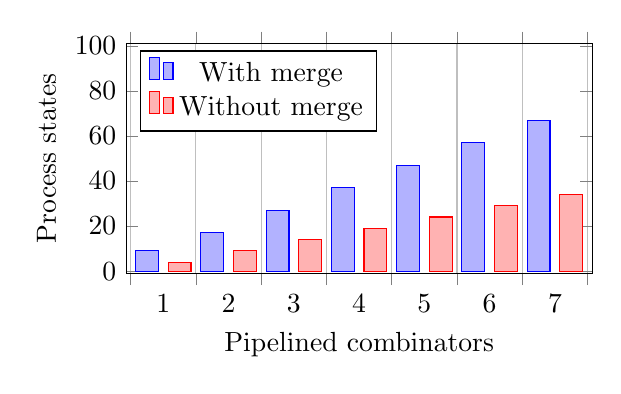
\begin{tikzpicture}
\begin{axis}[
% Hide the label on the second graph
        ylabel=Process states,
        xlabel=Pipelined combinators,
  ymin=0, ymax=100,
        enlargelimits=0.01,
        ybar interval=0.7,
  width=7.5cm, height=4.5cm,
        legend pos=north west,
]
\addplot coordinates {(1,9) (2,17) (3,27) (4,37) (5,47) (6,57) (7,67)   (8,1) };
\addplot coordinates {(1,4) (2,9) (3,14) (4,19) (5,24) (6,29) (7,34)    (8,1) };
\legend{With merge, Without merge};
\end{axis}
\end{tikzpicture}


To produce the above graph we programmatically generated dataflow networks for \emph{all possible} pipelined combinations of the @map@, @filter@, @scan@, @group@ and @merge@ combinators, and tried all possible fusion orders consiting of adjacent pairs of processes. The @merge@ combinator itself has two inputs, so only works at the very start of the pipeline --- we present result for pipelines with and without a @merge@ at the start. 

\subsection{Fusing Parallel Processes}
The following figure shows the number of states in the result when the various combinations of combinators are fused in parallel, for example, we might have a @map@ and a @filter@ processing the same input stream. In both cases the number of states in the result process grows linearly with the number of processes. In all combinations, with up to 7 processes there are less than 100 states in the result process.

\smallskip
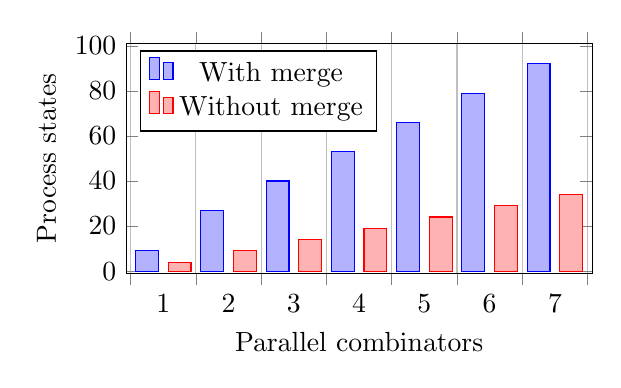
\begin{tikzpicture}
\begin{axis}[
        ylabel=Process states,
        xlabel=Parallel combinators,
  ymin=0, ymax=100,
        enlargelimits=0.01,
        ybar interval=0.7,
  width=7.5cm, height=4.5cm,
        legend pos=north west,
]
\addplot coordinates {(1,9) (2,27) (3,40) (4,53) (5,66) (6,79) (7,92)
  % Last bar doesn't show for some reason, so need to add a dummy value for the next one
    (8,1) };

\addplot coordinates {(1,4) (2,9) (3,14) (4,19) (5,24) (6,29) (7,34)    (8,1) };

\legend{With merge, Without merge};
\end{axis}
\end{tikzpicture}

The size of the result process is roughly what one would get when inlining the definitions of each of the original source processes. This is common with other systems based on inlining and/or template meta-programming, and is not prohibitive.


\eject{}
% -----------------------------------------------------------------------------
\subsection{Fusing Merges}

On the other hand, the following figure shows the results for a pathological case where the size of the output program is exponential in the number of input processes. The source dataflow networks consists of N merge processes, N+1 input streams, and a single output stream. The output of each merge process is the input of the next, forming a chain of merges. In source notation the network for N = 3 is @sOut = merge sIn1 (merge sIn2 (merge sIn3 sIn4))@.

\medskip
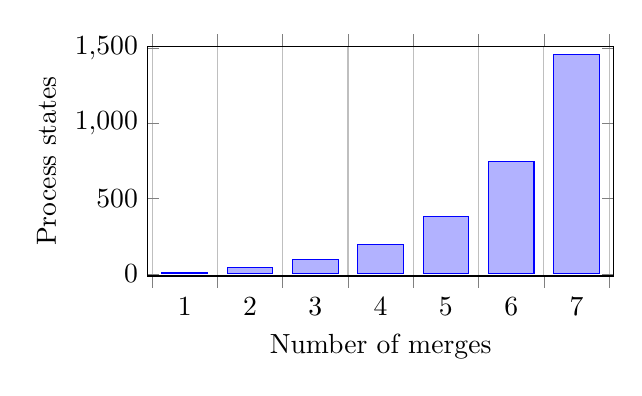
\begin{tikzpicture}
\begin{axis}[
        ylabel=Process states,
        xlabel=Number of merges,
%  ymode=log,
  ymin=0, ymax=1500,
        enlargelimits=0.01,
        ybar interval=0.7,
  width=7.5cm, height=4.5cm,
        legend pos=north west,
]
% These are the values for splitting.
% They are smaller than the 'chaining', but look much nicer on the linear graph.
\addplot coordinates {(1,9) (2,42) (3,97) (4,196) (5,383) (6,746) (7,1461)
  % (8,2880)
  (8,1)
  };

% These are the values for chaining
% \addplot coordinates {(1,4) (2,48) (3,194) (4,760) (5,2814) (6,10064) (7,1) };

\end{axis}
\end{tikzpicture}


When fusing two processes the fusion algorithm essentially compares every state in the first process with every state in the second, computing a cross product. During the fusion transform, as states in the result process are generated they are added to a finite map --- the @instrs@ field of the process definition. The use of the finite map ensures that identical states are always combined, but genuinely different states always make it into the result. 
In the worst case, fusion of two processes produces O($n*m$) different states, where $n$ and $m$ are the number of states in each. If we assume the two processes have about the same number of states then this is O($n^2$). Fusing the next process into this result yields O($n^3$), so overall the worst case number of states in the result will be O($n^k$), where $k$ is the number of processes fused. 

In the particular case of @merge@, the implementation has two occurrences of the @push@ instruction. During fusion, the states for the consuming process are inlined at each occurrence of @push@. These states are legitimately different because at each occurence of @push@ the input channels of the merge process are in different channel states, and these channel states are included in the overall process state.


\clearpage{}
%!TEX root = ../Appendix.tex
\clearpage{}

\section{Combinators}
\label{s:Combinators}
Here we show the definitions of some combinators. We start with simple combinators supported by most streaming systems, and progress to more interesting combinators. Some standard combinators such as @fold@, @take@ and @append@ are missing due to the infinite nature of our streams, but could be implemented with the finite stream extension. The fact that segmented versions of these combinators can be implemented is compelling evidence of this.

Many of these combinators take a ``default'' argument, which is used to initialise the heap, but the stored value is never actually read. Ideally these could be left unspecified, or the heap left uninitialised in cases where it is never read.

\subsection{Map}
The map combinator applies a function to every element of the stream. This is some more text.

\begin{alltt}
map 
 =  \(\lambda\) (f : \(\alpha \to \beta\)) (default : \(\alpha\))
      (sIn: Stream \(\alpha\)) (sOut: Stream \(\beta\)). 
    \(\nu\) (a: \(\alpha\)) (L0..L2: Label).
\end{alltt}
\begin{code}
    process
    { ins:    { sIn }
    , outs:   { sOut }
    , heap:   { a = default }
    , label:  L0
    , instrs: { L0 = pull sIn     a  L1 []
              , L1 = push sOut (f a) L2 []
              , L2 = drop sIn        L0 [] } }
\end{code}


% -----------------------------------------------------------------------------
\subsection{Filter}
Filter returns a new stream containing only the elements that satisfy some predicate.
\begin{alltt}
filter 
 =  \(\lambda\) (f : \(\alpha \to\) Bool) (default : \(\alpha\))
      (sIn: Stream \(\alpha\)) (sOut: Stream \(\alpha\)). 
    \(\nu\) (a: \(\alpha\)) (L0..L3: Label).
\end{alltt}
\begin{code}
    process
    { ins:    { sIn }
    , outs:   { sOut }
    , heap:   { a = default }
    , label:  L0
    , instrs: { L0 = pull sIn  a     L1 []
              , L1 = case   (f a)    L2 []  L3 []
              , L2 = push sOut a     L3 []
              , L3 = drop sIn        L0 [] } }
\end{code}


\vspace{12em}
% -----------------------------------------------------------------------------
\subsection{Partition}
Partition is similar to filter, but has two output streams: those that satisfy the predicate, and those that do not. Partition is an inherently push-based operation, and cannot be supported by pull streams without buffering.
\begin{alltt}
partition 
 =  \(\lambda\) (f : \(\alpha \to\) Bool) (default : \(\alpha\))
      (sIn:   Stream \(\alpha\))
      (sOut1: Stream \(\alpha\)) (sOut2: Stream \(\alpha\)). 
    \(\nu\) (a: \(\alpha\)) (L0..L4: Label).
\end{alltt}
\begin{code}
    process
    { ins:    { sIn }
    , outs:   { sOut1, sOut2 }
    , heap:   { a = default }
    , label:  L0
    , instrs: { L0 = pull sIn   a    L1 []
              , L1 = case    (f a)   L2 []  L3 []
              , L2 = push sOut1 a    L4 []
              , L3 = push sOut2 a    L4 []
              , L4 = drop sIn        L0 [] } }
\end{code}


% -----------------------------------------------------------------------------
\subsection{Zip}
Zip, or zip-with, pairwise combines two input streams.
Zipping is an inherently pull-based operation.

\begin{alltt}
zipWith 
 =  \(\lambda\) (f : \(\alpha \to \beta \to \gamma\)) (default1 : \(\alpha\)) (default2 : \(\beta\))
      (sIn1: Stream \(\alpha\)) (sIn2: Stream \(\beta\))
      (sOut: Stream \(\gamma\)). 
    \(\nu\) (a: \(\alpha\)) (b : \(\beta\)) (L0..L4: Label).
\end{alltt}
\begin{code}
    process
    { ins:    { sIn1, sIn2 }
    , outs:   { sOut }
    , heap:   { a = default1, b = default2 }
    , label:  L0
    , instrs: { L0 = pull sIn1 a       L1 []
              , L1 = pull sIn2 b       L2 []
              , L2 = push sOut (f a b) L3 []
              , L3 = drop sIn1         L4 []
              , L4 = drop sIn2         L0 [] } }
\end{code}


% -----------------------------------------------------------------------------
\subsection{Scan}
Scan is similar to a fold, but instead of returning a single value at the end, it returns an intermediate value for each element of the stream.

\begin{alltt}
scan 
 =  \(\lambda\) (k : \(\alpha \to \beta \to \beta\)) (z : \(\beta\)) (default : \(\alpha\))
      (sIn: Stream \(\alpha\)) (sOut: Stream \(\beta\)).
    \(\nu\) (a: \(\alpha\)) (s : \(\beta\)) (L0..L2: Label).
\end{alltt}
\begin{code}
    process
    { ins:    { sIn  }
    , outs:   { sOut }
    , heap:   { a = default, s = z }
    , label:  L0
    , instrs: { L0 = pull sIn  a   L1 []
              , L1 = push sOut s   L2 [ s = f a s ]
              , L2 = drop sIn      L0 [] } }
\end{code}


% -----------------------------------------------------------------------------
\subsection{Segmented Fold}
Segmented fold performs a fold over each nested stream, using a segmented representation.
Here we are representing nested streams using one stream for the lengths of each substream, and another stream containing the values.
The output stream has the same rate as the lengths stream.
It reads a count (@c@) from the lengths stream, setting the fold state to zero (@z@).
Then it reads count times from the values stream, updating the fold state.
Afterwards, it pushes the final fold state, and continues to read a new count.

\begin{alltt}
folds 
 =  \(\lambda\) (k : \(\alpha \to \beta \to \beta\)) (z : \(\beta\)) (default : \(\alpha\))
      (sLens: Stream Nat) (sVals: Stream \(\alpha\))
      (sOut:  Stream \(\beta\)).
    \(\nu\) (c : Nat) (a: \(\alpha\)) (s : \(\beta\)) (L0..L5: Label).
\end{alltt}
\begin{code}
    process
    { ins:    { sLens, sVals }
    , outs:   { sOut }
    , heap:   { c = 0, a = default, s = z }
    , label:  L0
    , instrs: { L0 = pull sLens c   L1 [ s = z ]
              , L1 = case (c > 0)   L2 []  L4 []
              , L2 = pull sVals a   L3 []
              , L3 = drop sVals     L1 [ c = c - 1
                                       , s = k s a ]
              , L4 = push sOut  s   L5 []
              , L5 = drop sLens     L0 [] } }
\end{code}


% -----------------------------------------------------------------------------
\subsection{Segmented Take}
Segmented take computes an @n@-length prefix of each nested stream.
It starts by reading a count from the lengths stream, then copies at most @n@ elements.
If there are leftovers, it pulls and discards them, then pulls the next length.

\begin{alltt}
takes 
 =  \(\lambda\) (n : Nat) (default : \(\alpha\))
      (sLens: Stream Nat) (sVals: Stream \(\alpha\))
      (oLens: Stream Nat) (oVals: Stream \(\alpha\)).
    \(\nu\) (c : Nat) (take : Nat) (ix : Nat) (a: \(\alpha\))
      (L0..L9: Label).
\end{alltt}
\begin{code}
    process
    { ins:    { sLens, sVals }
    , outs:   { oLens, oVals }
    , heap:   { c = 0, take = 0, ix = 0, a = default }
    , label:  L0
    , instrs: { L0 = pull sLens c     L1 
                          [ ix = 0, take = min count n ]
              , L1 = push oLens take  L2 []
              , L2 = case (ix < take) L3 []  L6 []
              , L3 = pull sVals a     L4 []
              , L4 = push oVals a     L5 []
              , L5 = drop sVals       L2 [ix = ix+1]
              , L6 = case (ix < c)    L7 []  L9 []
              , L7 = pull sVals a     L8 []
              , L8 = drop sVals       L6 [ix = ix+1]
              , L9 = drop sLens       L0 [] } }
\end{code}


% -----------------------------------------------------------------------------
\subsection{Segmented Append}
Segmented append takes two segmented streams as input, and appends each nested stream.
It starts by reading a length from both lengths streams into @a@ and @b@, and pushes the sum of both lengths.
It then copies over @a@ elements from the first values stream, then copies over @b@ elements from the second values stream.

\begin{alltt}
appends 
 =  \(\lambda\) (default : \(\alpha\))
      (aLens: Stream Nat) (aVals: Stream \(\alpha\))
      (bLens: Stream Nat) (bVals: Stream \(\alpha\))
      (oLens: Stream Nat) (oVals: Stream \(\alpha\)).
    \(\nu\) (a : Nat) (b : Nat) (v: \(\alpha\)) (L0..L12: Label).
\end{alltt}
\begin{code}
    process
    { ins:    { aLens, aVals, bLens, bVals }
    , outs:   { oLens, oVals }
    , heap:   { a = 0, b = 0, v = default }
    , label:  L0
    , instrs: { L0  = pull aLens  a    L1 []
              , L1  = pull bLens  b    L2 []
              , L2  = push oLens (a+b) L3 []

              , L3  = case (a > 0)     L4 []  L7 []
              , L4  = pull aVals v     L5 []
              , L5  = push oVals v     L6 []
              , L6  = drop aVals       L3 [ a = a-1 ]

              , L7  = case (b > 0)     L8 []  L11[]
              , L8  = pull bVals v     L9 []
              , L9  = push oVals v     L10[]
              , L10 = drop bVals       L7 [ b = b-1 ]

              , L11 = drop aLens        L12[]
              , L12 = drop bLens        L0 [] } }
\end{code}



% \bibliography{Main}

\end{document}

